% --- UNIVERSAL PREAMBLE BLOCK ---
\documentclass[11pt, a4paper]{article}
\usepackage[a4paper, top=2.5cm, bottom=2.5cm, left=2cm, right=2cm]{geometry}

\usepackage[english]{babel}
\usepackage{graphicx}
\usepackage{hyperref}

% --- DOCUMENT INFO ---
\title{\textbf{MAT306: Normal Mode Analysis of a Nanoparticle}}
\author{Ahmet Ekiz}
\date{\today}

\begin{document}

\begin{titlepage}
  \centering
  \vspace*{3cm}

  {\LARGE \textbf{MAT306}\\[0.4cm]}
  {\Huge \textbf{Normal Mode Analysis of a Nanoparticle}\\[1.5cm]}

  {\Large Homework Report\\[2cm]}

  {\large \textbf{Student:} Ahmet Ekiz\\[0.3cm]}
  {\large \textbf{Date:} \today}

  \vfill
\end{titlepage}

\tableofcontents
\newpage

\section*{Initial Calculations}
\addcontentsline{toc}{section}{Initial Calculations}

% ==========================================
% QUESTION 1
% ==========================================

\textbf{Start by visualizing and inspecting your system. Provide a VMD visualization snapshot of your system of choice in a representation that is clear. State where this nanoparticle is used/why it has caught your interest.}
\vspace{0.5cm}

For this assignment, I have selected \textbf{QDNP015} from the ViNAS toolbox. This nanoparticle is a Cadmium-Telluride (CdTe) core quantum dot, comprised of 2,805 total atoms. 

\begin{figure}[htbp]
  \centering
  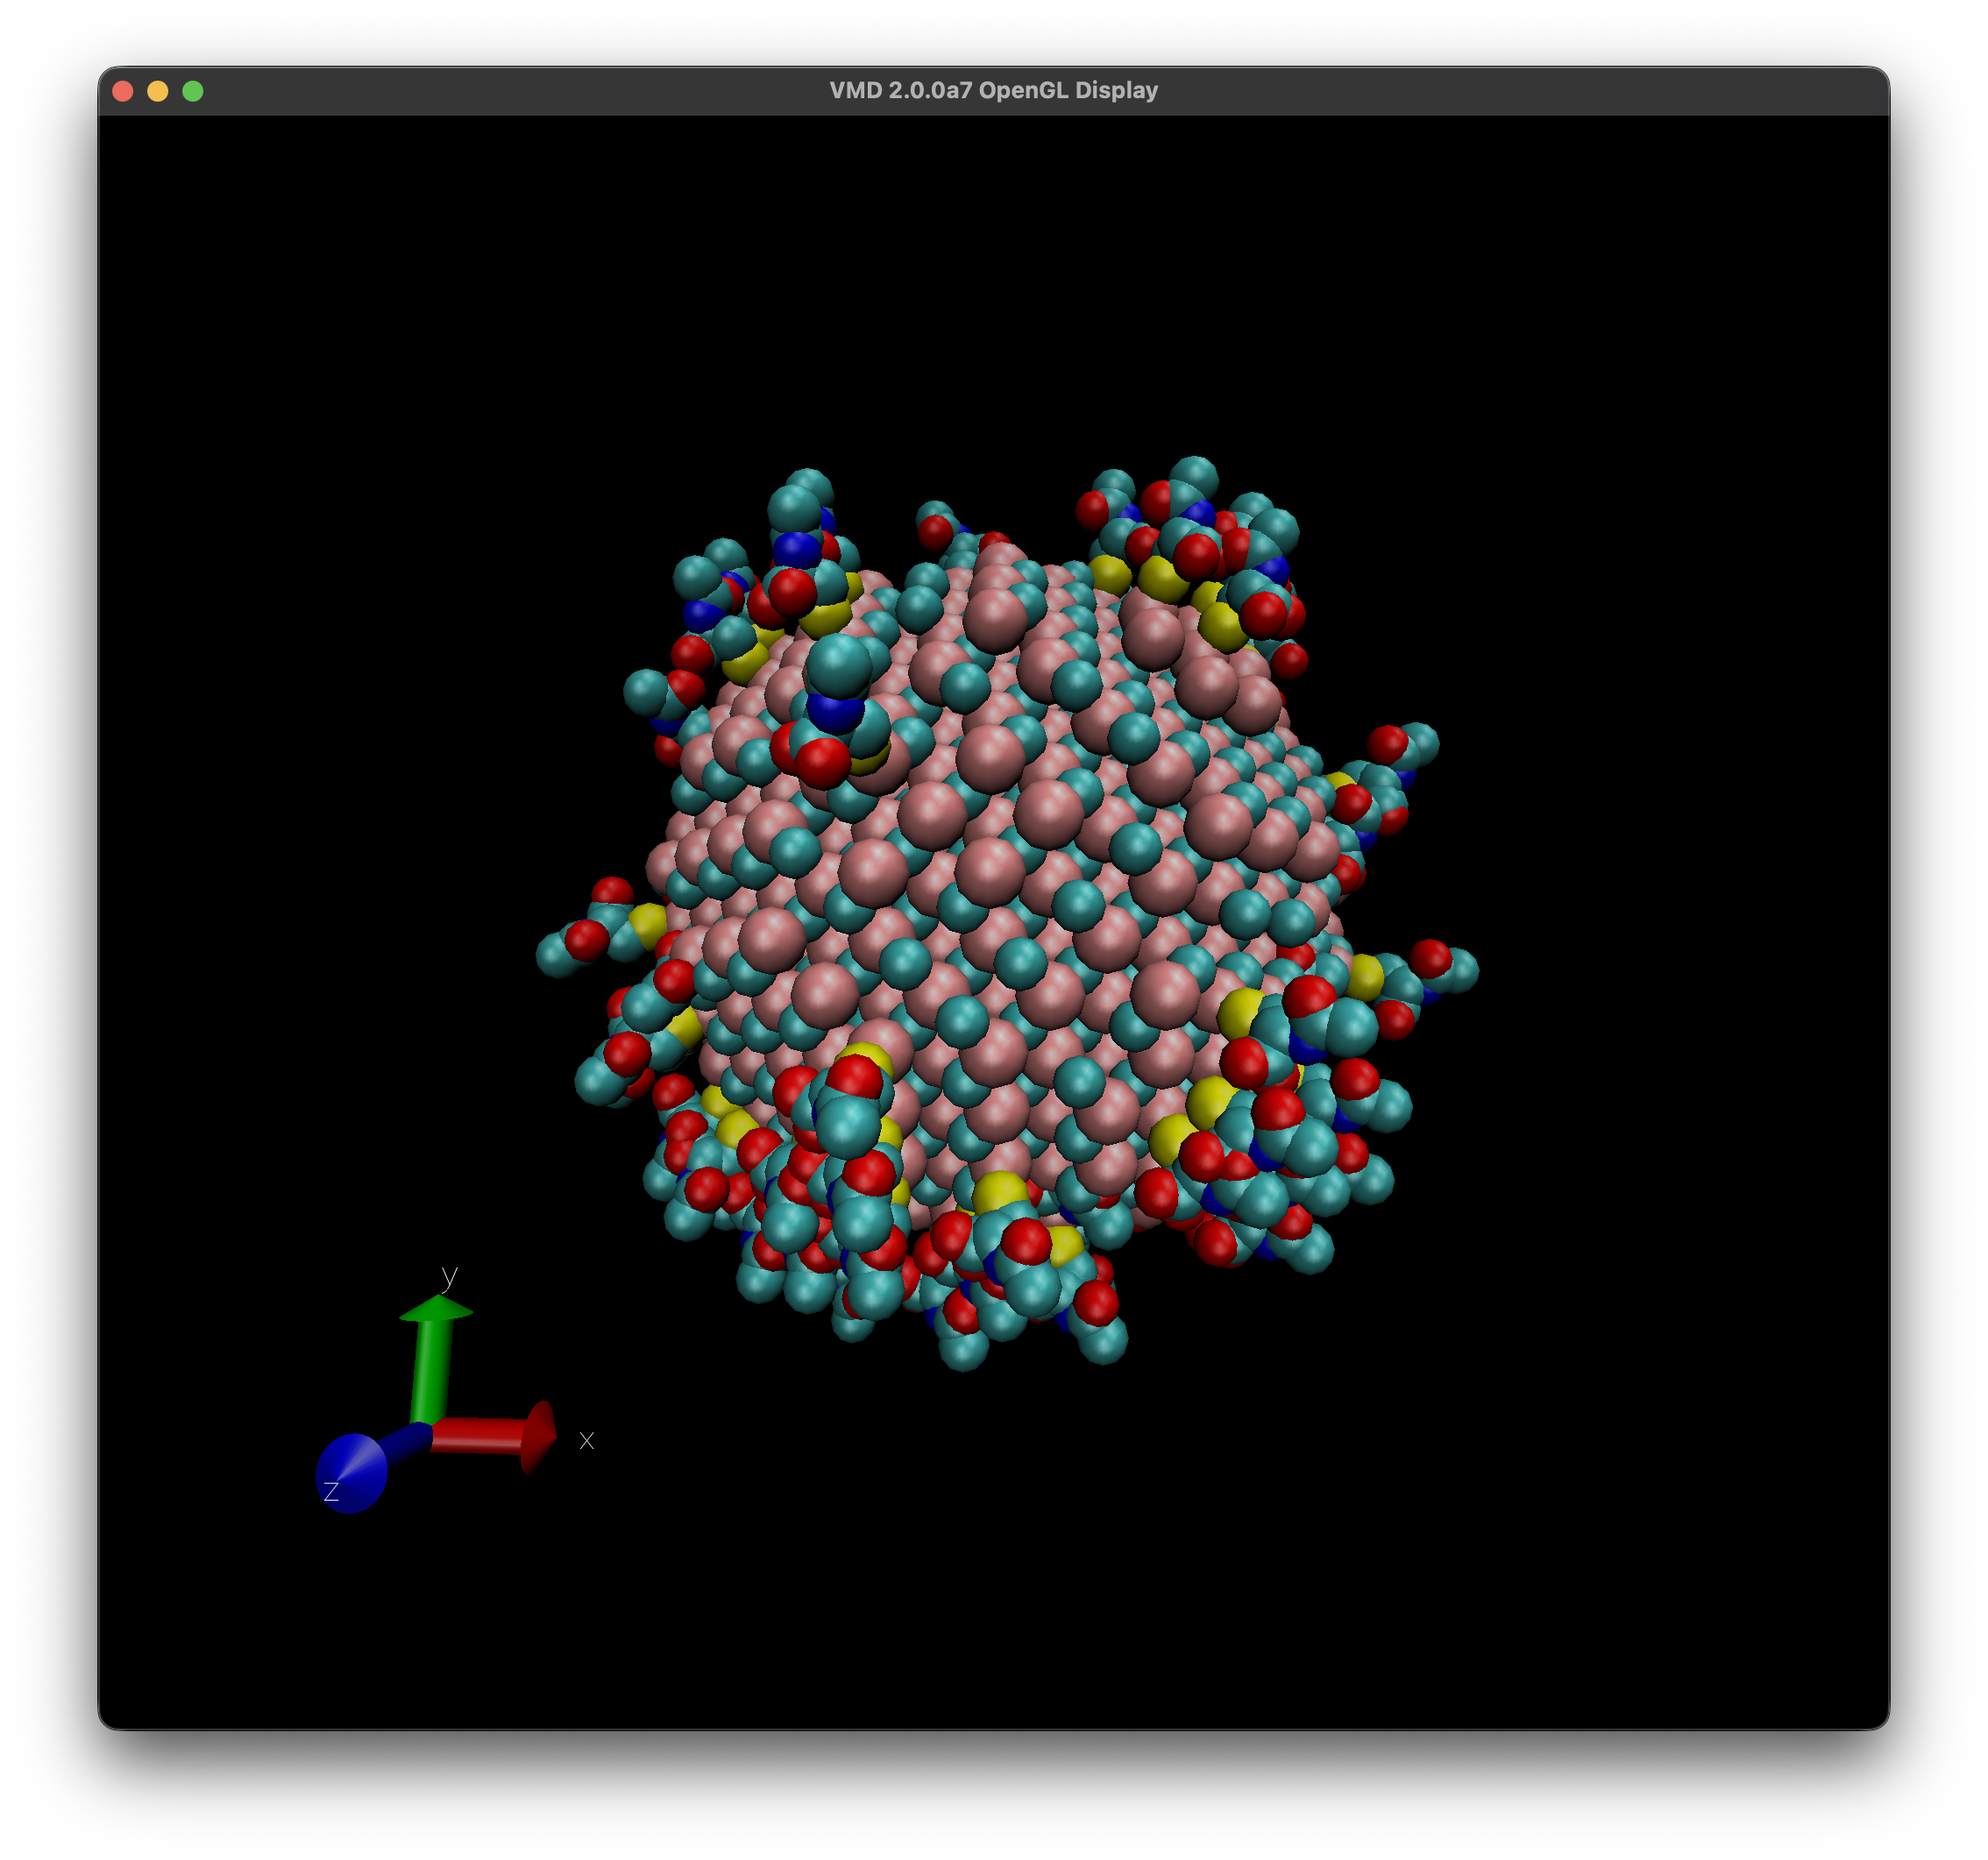
\includegraphics[width=0.8\textwidth]{Figure0-1.png}
  \caption{VMD visualization of the QDNP015 Cadmium-Telluride (CdTe) quantum dot core and surface ligands.}
  \label{fig:vmd_snapshot}
\end{figure}

\textbf{Motivation and Real-World Application:}\\
I chose quantum dots (QDs) as my nanoparticle of interest because they represent a fascinating class of nanomaterials with unique size-dependent optical and electronic properties. They are widely used in various applications, including display technologies (QLED TVs), biological imaging, and solar cells. The specific CdTe quantum dot I selected is big enough to exhibit complex vibrational dynamics while still being computationally manageable for normal mode analysis.

\newpage

% ==========================================
% QUESTION 1
% ==========================================

\vspace{0.5cm}
\section*{Initial Calculations (Continued)}
\addcontentsline{toc}{section}{Initial Calculations (Continued)}

\textbf{You will have to coarse-grain your system because there are too many atoms even in a nanoparticle. Make sure you coarse-grain on the same type of atom; this should not be too hard since all these systems have a repetition of sorts in them. Make sure there is at least 4 \AA\ on the closest pair of nodes.}
\vspace{0.5cm}

To reduce the computational complexity of the normal mode analysis, the QDNP015 system was coarse-grained. Instead of calculating the physical interactions for all 2,805 individual atoms (which would be highly resource-intensive), a single element type was chosen to represent the simplified structural skeleton, or "nodes", of the network model.

I selected the \textbf{Cadmium (Cd)} atoms to serve as the nodes for this coarse-grained model. The QDNP015 core possesses 902 Cadmium atoms. 

To verify that this selection meets the assignment criteria for node spacing, the distance between adjacent Cadmium atoms in the nanoparticle's crystal lattice was measured using VMD's \texttt{Mouse -> Label -> Bonds} tool. The measurement revealed that the distance between the closest pair of adjacent Cadmium nodes is approximately \textbf{4.68 \AA}. 

Because 4.68 \AA\ is strictly greater than the required minimum threshold of 4.0 \AA, coarse-graining on the Cadmium atoms successfully satisfies the assignment requirements and provides a valid, well-spaced structural framework for building the subsequent Gaussian and Anisotropic Network Models.

\begin{figure}[htbp]
  \centering
  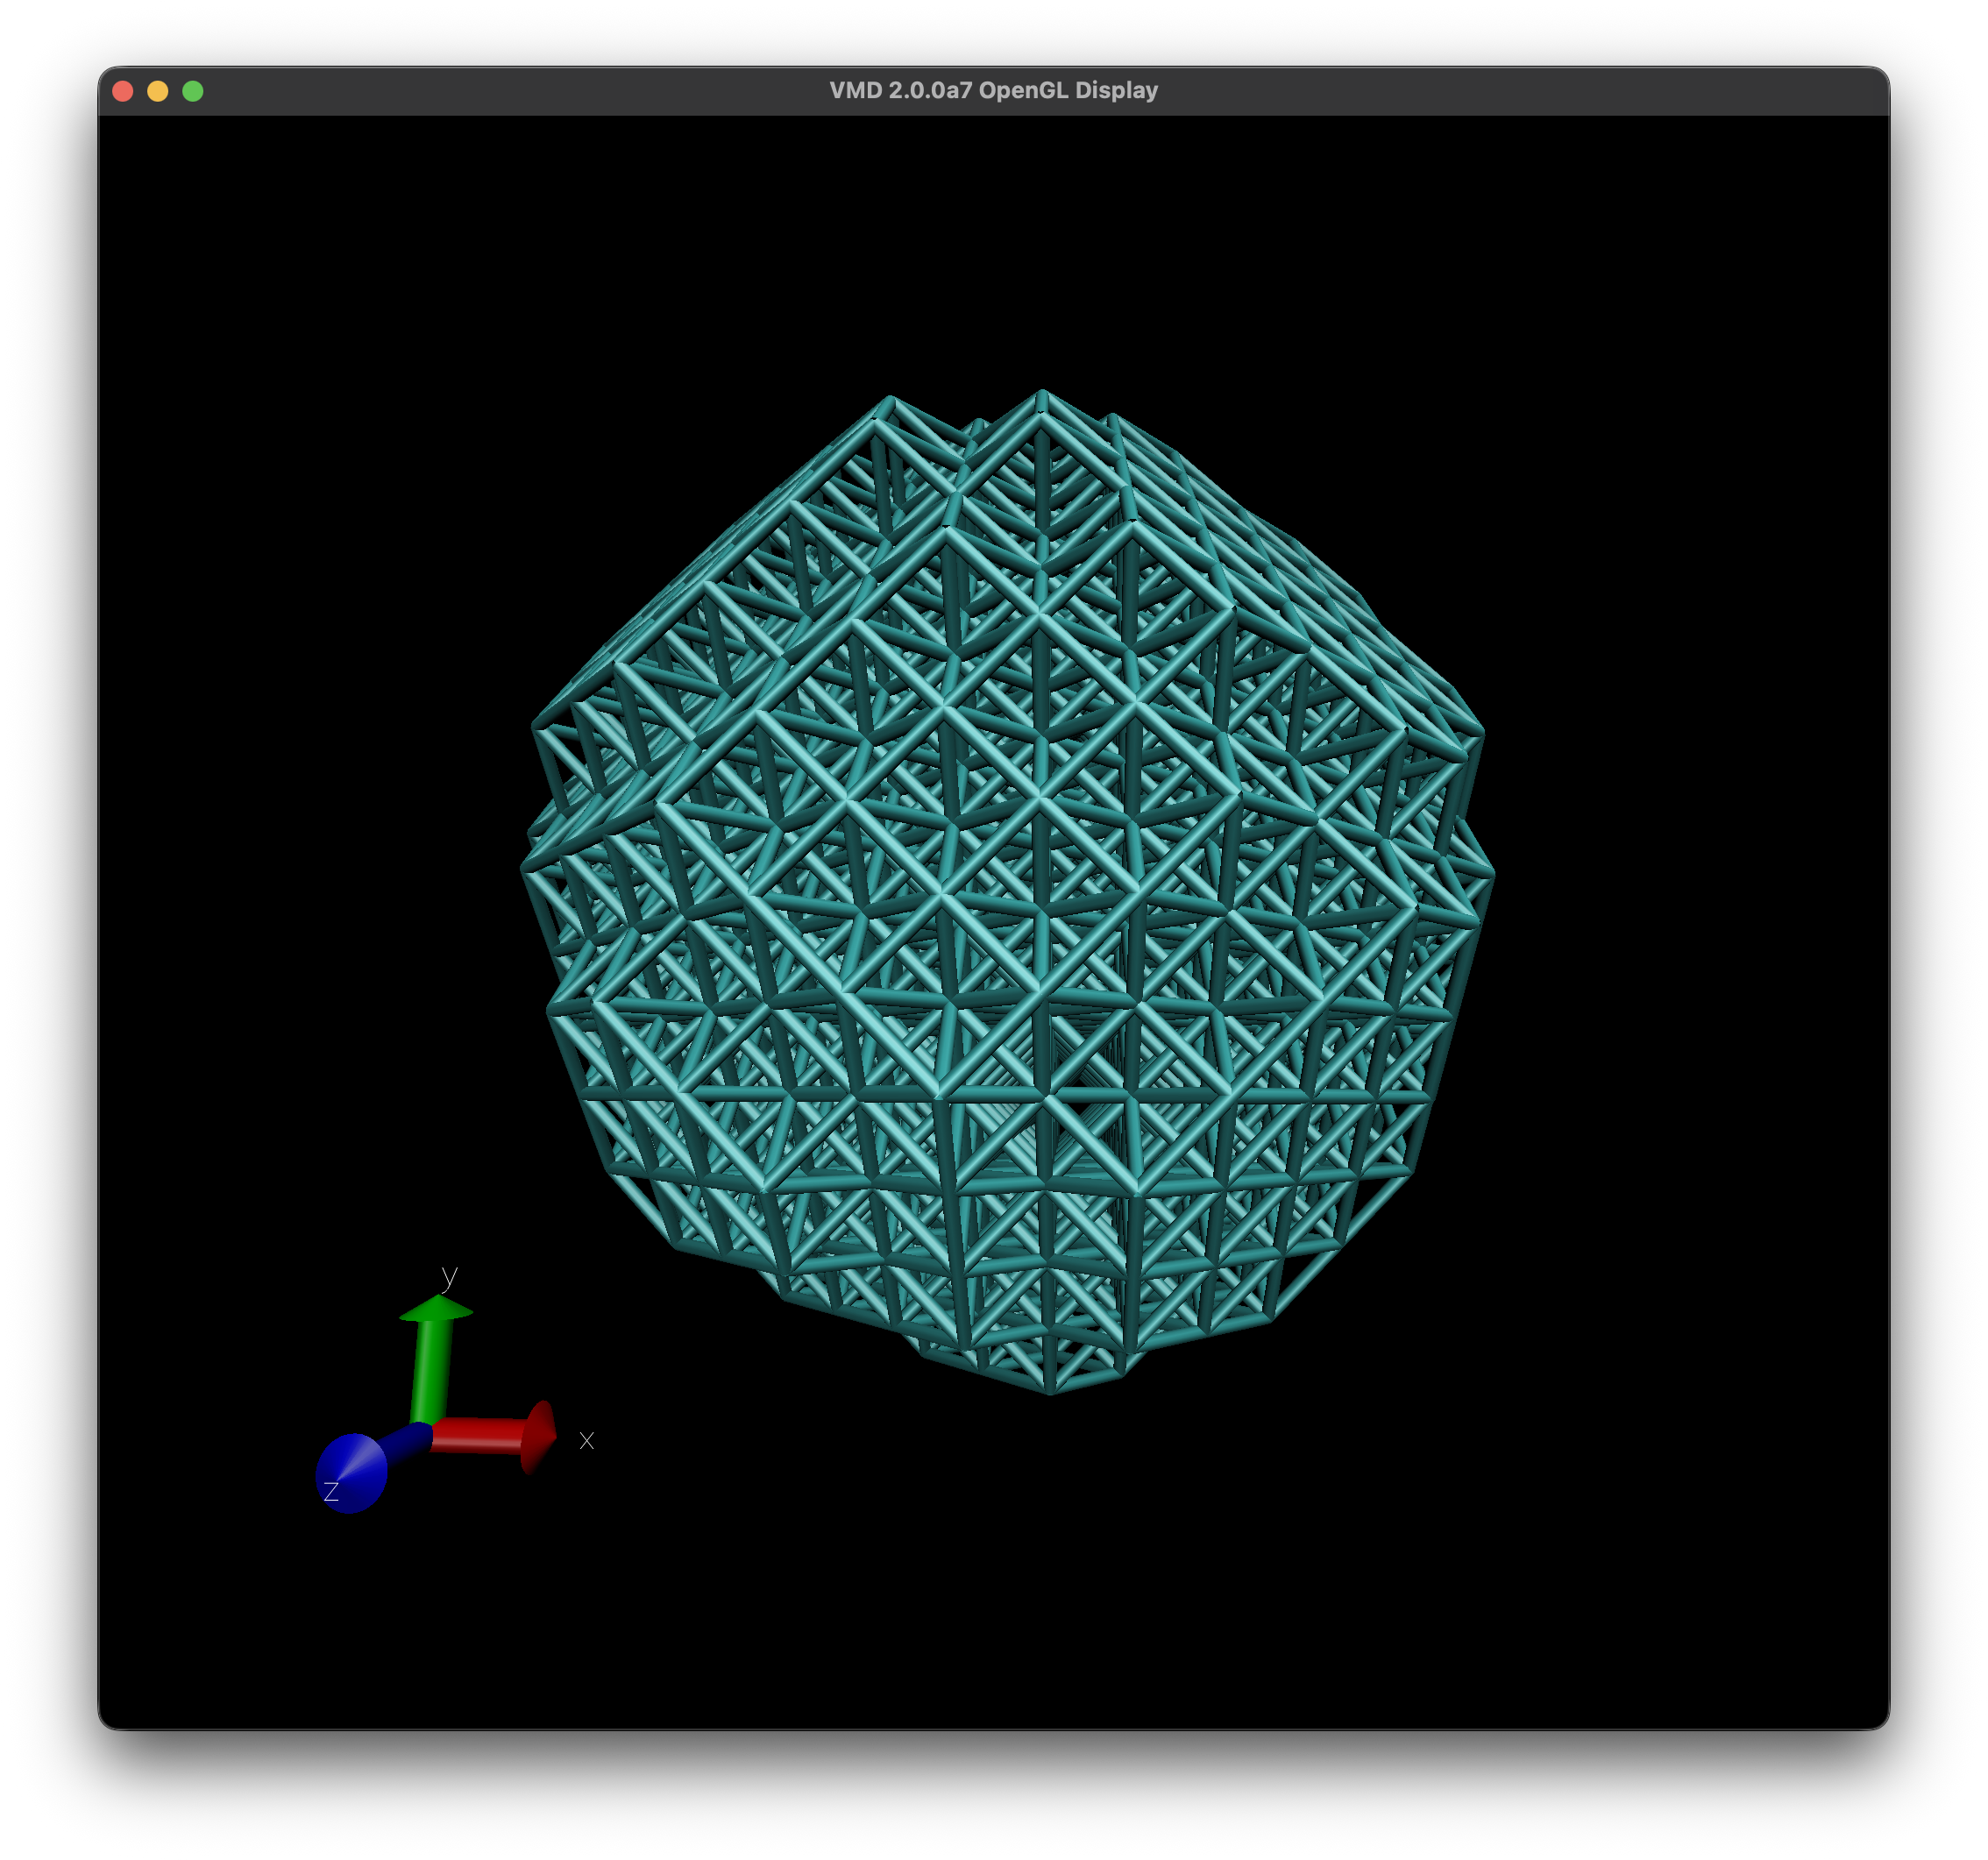
\includegraphics[width=0.45\textwidth]{Figure1-1.png}
  \hfill
  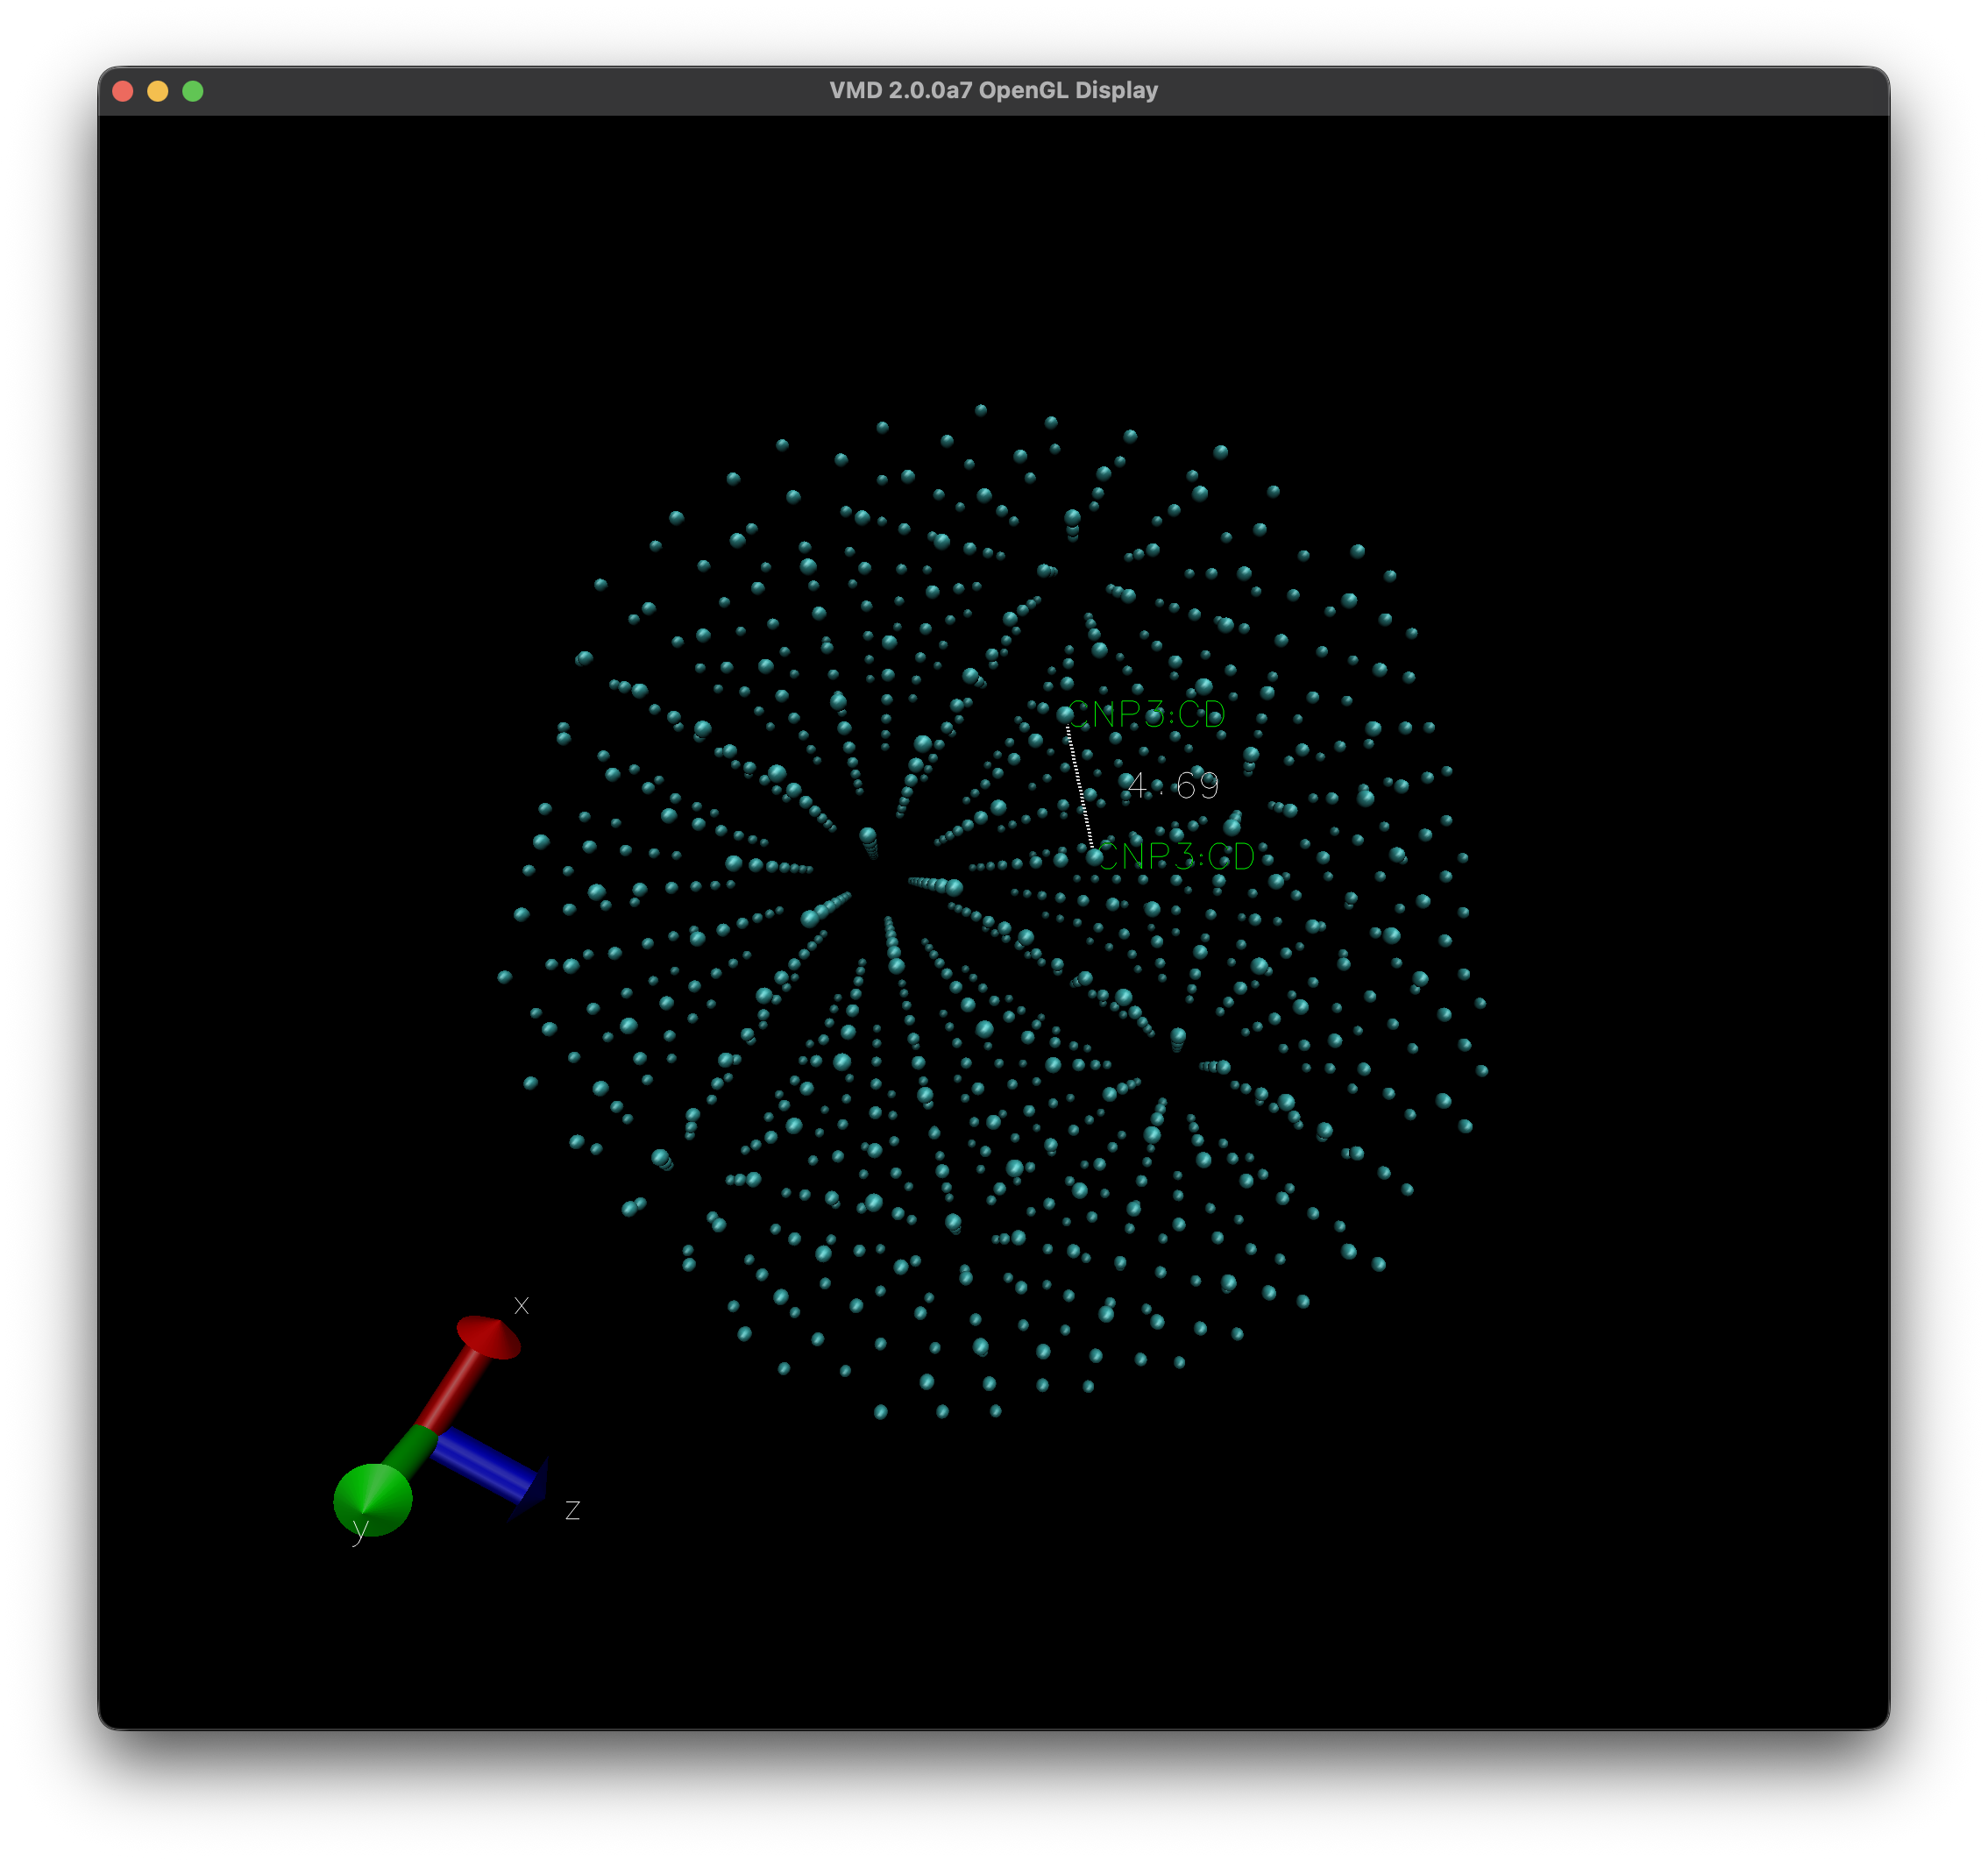
\includegraphics[width=0.45\textwidth]{Figure1-2.png}
  \caption{Measurement of distance between adjacent Cadmium nodes using VMD.}
  \label{fig:node_distance}
\end{figure}

\newpage

% ==========================================
% QUESTION 2 & 3
% ==========================================
\section*{GNM Construction and Results}
\addcontentsline{toc}{section}{GNM Construction and Results}

\textbf{Make a first guess on what the cutoff distance ($R_c$) might be. For this simple scenario, we will take all interactions between pairs of nodes to have equal spring constant in all our models. Construct the Gaussian Network Model (GNM) using the $R_c$ you selected. You may choose to update $R_c$ after an initial analysis (see next item)}
\vspace{0.5cm}

Based on my visual measurement in VMD, the distance between adjacent Cadmium nodes is 4.68 \AA. If the cutoff distance is set too tightly (e.g., $< 5.0$ \AA), the network risks becoming fragmented or under-connected. Therefore, I made a first guess of \textbf{$R_c = 6.0$ \AA} to give the enough buffer. This provides a sufficient buffer to capture the primary nearest-neighbor bonds while establishing a robust, interconnected web of virtual springs for the Gaussian Network Model (GNM) without making the matrix overly dense. 

\vspace{1.5cm}

\newpage

\textbf{Make a list of the eigenvalues of your molecule. How many non-zero eigenvalues did you expect, and did your findings agree with your expectations? What other properties do your eigenvalues present? Provide a plot of eigenvalue vs. node index with your final selected cutoff distance which you should clearly indicate on the plot.}
\vspace{0.5cm}

\textbf{Expectations vs. Findings:}\\
For a 1-dimensional model like the GNM, the system computes one degree of freedom per node. Because there is exactly 1 zero eigenvalue corresponding to the whole-system translation, the expected number of non-zero eigenvalues is $N - 1$. With $N = 902$ Cadmium nodes, I expected exactly \textbf{901} non-zero eigenvalues. 

Initially, running ProDy's default calculation yielded only 20 modes due to standard computational limits. However, upon forcing the calculation of all modes (\texttt{n\_modes='all'}), my findings yielded exactly 901 non-zero eigenvalues, perfectly agreeing with my mathematical expectations.

\vspace{0.5cm}
\textbf{List and Properties of Eigenvalues:}\\
The calculated eigenvalues represent the relative stiffness/frequency of the vibrational modes:
\begin{itemize}
    \item Mode 1 (Slowest): $\lambda_1 = 0.274187$
    \item Mode 2: $\lambda_2 = 0.274187$
    \item \dots
    \item Mode 901 (Fastest): $\lambda_{901} = 15.803611$
\end{itemize}
The eigenvalues are sorted in ascending order. The lowest eigenvalues ($\sim 0.27$) represent "soft" modes, which physically translate to large-scale, global, and highly cooperative structural movements (such as the entire nanoparticle bending or breathing). The highest eigenvalues ($\sim 15.8$) represent "stiff" modes, corresponding to extremely fast, tiny, localized twitches deep within the densely packed core.

\newpage
\begin{figure}[htbp]
  \centering
  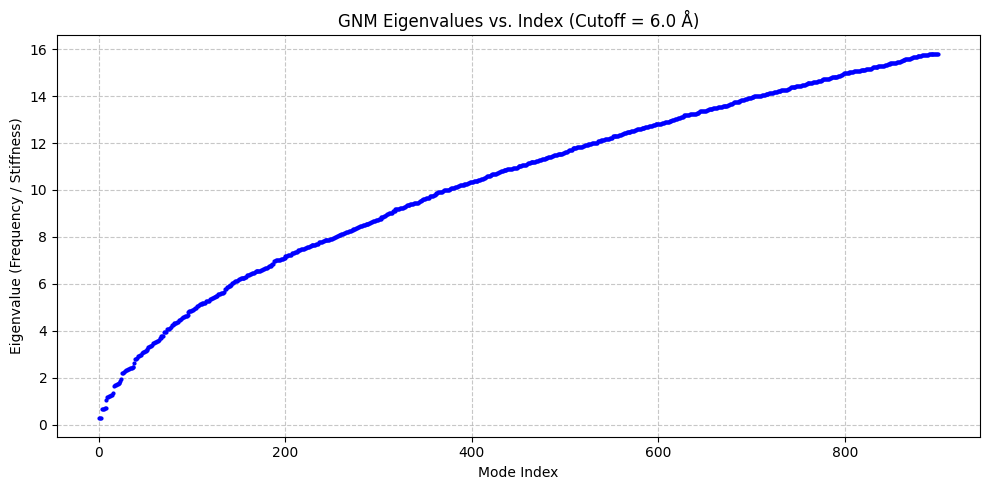
\includegraphics[width=0.8\textwidth]{Figure3-1.png}
  \caption{GNM Eigenvalues vs. Mode Index using a cutoff distance of $R_c = 6.0$ \AA.}
  \label{fig:gnm_eigenvalues}
\end{figure}

% ==========================================
% QUESTION 4
% ==========================================
\newpage

\newpage
\section*{GNM Construction and Results (Continued)}
\addcontentsline{toc}{section}{GNM Construction and Results (Continued)}

\textbf{Plot the eigenvector that corresponds to the slowest non-zero eigenvalue; i.e. provide eigenvalue vs. node index plot. Describe its properties.}
\vspace{0.5cm}

\begin{figure}[htbp]
  \centering
  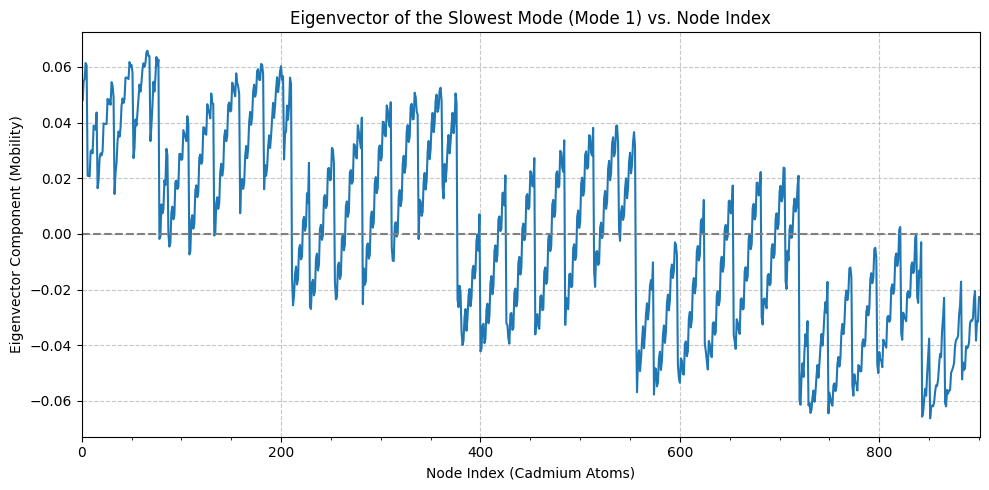
\includegraphics[width=0.8\textwidth]{Figure4-1.png}
  \caption{Eigenvector components of the slowest GNM mode (Mode 1) plotted against Node Index.}
  \label{fig:gnm_eigenvector}
\end{figure}

\vspace{0.5cm}
\textbf{Properties of the Slowest Eigenvector:}\\
The plot of the slowest mode (Mode 1) displays highly structured, cooperative motion rather than random individual fluctuations. The distinct "block-like" regions—where large consecutive groups of node indices are mostly positive (e.g., indices 0–200) or mostly negative (e.g., indices 550–700)—suggest that entire domains or hemispheres of the nanoparticle are moving together in opposite directions.

Because the 1D mathematical node index (0–901) represents a coordinate sequence that sweeps across the 3D volume of the nanoparticle layer-by-layer, these blocks correspond to physical "slices" of the sphere. Within these slices, the jagged, rapid spikes occur as the numbering sequence alternates between unconstrained surface atoms and denser interior atoms. The nodes with the highest absolute mobility (the extreme peaks and deep valleys) represent the flexible surface atoms, while the nodes hovering near the zero-line represent the highly stable, structural core acting as a stationary hinge for this global bending motion.

\newpage

% ==========================================
% QUESTION 5
% ==========================================
\section*{GNM Construction and Results (Continued)}
\addcontentsline{toc}{section}{GNM Construction and Results (Continued)}

\textbf{Display both your $\Gamma$ matrix and its inverse in side-by-side graphs. Comment on your understanding of what is plotted.}
\vspace{0.5cm}

\begin{figure}[htbp]
  \centering
  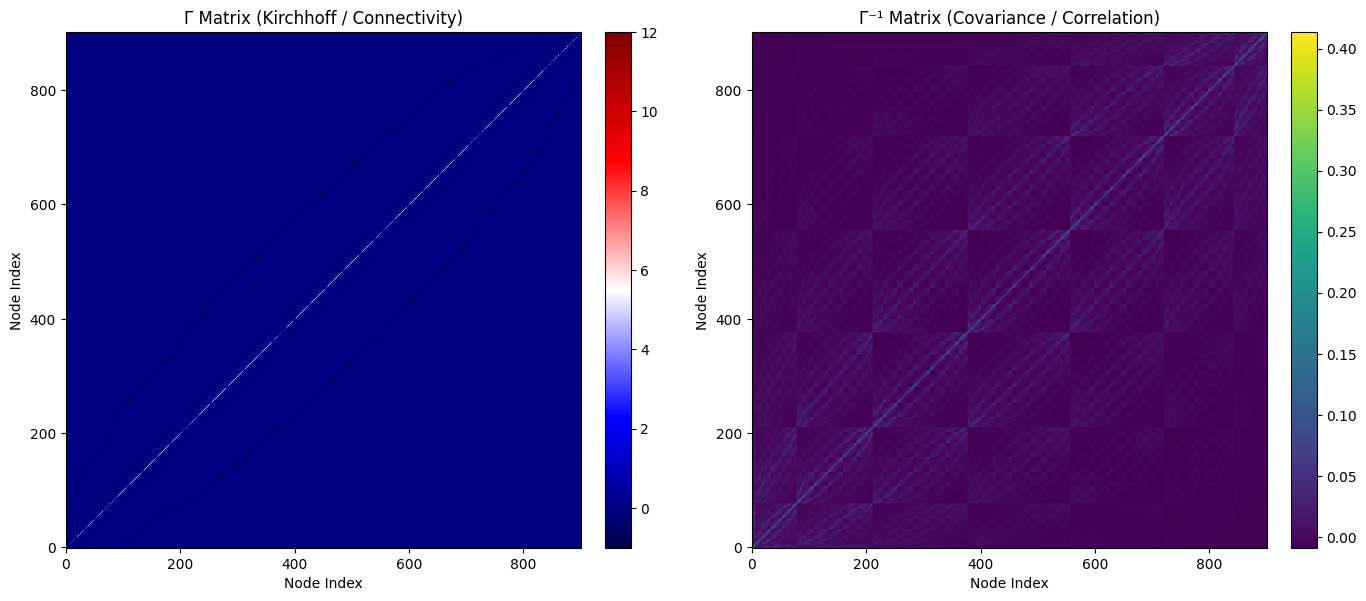
\includegraphics[width=0.8\textwidth]{Figure5-1.png}
  \caption{Left: The $\Gamma$ (Kirchhoff) matrix showing direct node connectivity. Right: The $\Gamma^{-1}$ (Covariance) matrix showing global node correlations.}
  \label{fig:gnm_matrices}
\end{figure}

\vspace{0.5cm}
\textbf{Understanding of the Plotted Matrices:}\\
The $\Gamma$ (Kirchhoff) matrix displays the direct physical connectivity of the network. The bright central diagonal represents the high number of local neighbors (the node degree) for each Cadmium atom within the 6.0 \AA\ cutoff, while the dark regions indicate a lack of direct connections between distant nodes. 

Conversely, the $\Gamma^{-1}$ (Covariance) matrix reveals the global dynamics and cross-correlations of the entire system. Its exceptionally bright central diagonal shows perfect auto-correlation (a node's movement relative to itself). More importantly, the repeating, grid-like checkerboard patterns in the off-diagonal regions demonstrate long-range structural correlations. These periodic bands ("echoes") occur because nodes that are far apart in the 1D mathematical index sequence are physically adjacent to one another on the 3D spherical surface of the quantum dot, causing their movements to be highly correlated.

\newpage

% ==========================================
% QUESTION 6
% ==========================================
\section*{ANM Construction and Results}
\addcontentsline{toc}{section}{ANM Construction and Results}

\textbf{Construct the Anisotropic Network Model (ANM). You may need to update $R_c$ again (why?) Clearly state your $R_c$. Make a list of the eigenvalues of your molecule. How many non-zero eigenvalues did you expect, and did your findings agree with your expectations? What other properties do your eigenvalues present? Provide a plot of eigenvalue vs. index with your final selected cutoff distance which you should clearly indicate on the plot.}
\vspace{0.5cm}

\textbf{Updating $R_c$ for ANM:}\\
I updated the cutoff distance to \textbf{$R_c = 10.0$ \AA}. For proteins, increasing the cutoff when transitioning from GNM to ANM is typically necessary because the ANM accounts for 3D spatial fluctuations (x, y, and z degrees of freedom per node), making the structural network inherently more flexible than the 1D GNM. A tighter cutoff can cause the protein network to fragment, producing excess zero eigenvalues and unphysical ``floppy'' modes.

However, an important observation for our nanoparticle is that, unlike proteins, reducing the cutoff distance back to 6.0 \AA\ does \textit{not} cause fragmentation or change the number of non-zero eigenvalues. The ANM at $R_c = 6.0$ \AA\ still yields exactly the expected 2700 non-zero modes with zero excess trivial eigenvalues. The only effect of changing the cutoff is a scaling of the overall stiffness of the system: a smaller cutoff produces lower eigenvalues (softer modes) because fewer virtual springs connect each node, while a larger cutoff increases stiffness uniformly. This behavior is a direct consequence of the tightly packed, highly symmetric crystal lattice structure of the CdTe quantum dot, which ensures that the network remains fully connected even at the tighter 6.0 \AA\ cutoff. For the final ANM analysis presented below, the cutoff of $R_c = 10.0$ \AA\ is retained as it provides a denser, more physically realistic spring network.

\textbf{Expectations vs. Findings:}\\
For an ANM, each node has 3 degrees of freedom, resulting in $3N$ total dimensions. Because a 3D object has 6 trivial degrees of freedom (3 translations and 3 rotations), the expected number of non-zero eigenvalues is $3N - 6$. With 902 nodes, I expected $3(902) - 6 = \textbf{2700}$ non-zero eigenvalues. My calculations yielded exactly 2700 modes, perfectly agreeing with expectations.

\textbf{Properties of Eigenvalues:}\\
The lowest eigenvalues represent the softest modes (large-scale, global 3D deformations like twisting or breathing). As the mode index increases, the eigenvalues increase rapidly, representing progressively stiffer, higher-frequency, and more localized atomic vibrations deep within the nanoparticle core.

\begin{figure}[htbp]
  \centering
  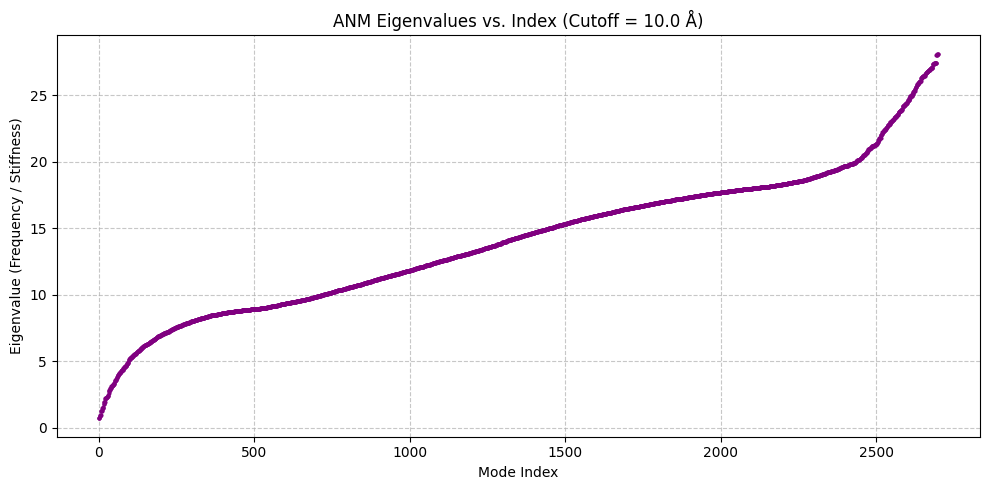
\includegraphics[width=0.8\textwidth]{Figure6-1.png}
  \caption{ANM Eigenvalues vs. Mode Index using a cutoff distance of $R_c = 10.0$ \AA.}
  \label{fig:anm_eigenvalues}
\end{figure}

\newpage

% ==========================================
% QUESTION 7
% ==========================================
\section*{ANM Construction and Results (Continued)}
\addcontentsline{toc}{section}{ANM Construction and Results (Continued)}

\textbf{Discuss the properties of the eigenvector that corresponds to the slowest non-zero eigenvalue.}
\vspace{0.5cm}

The eigenvector corresponding to the slowest non-zero mode (Mode 1) in the ANM represents the most highly cooperative, lowest-energy 3D deformation of the nanoparticle. Unlike the GNM eigenvector which contains $N$ components, this ANM eigenvector contains $3N$ components (2,706 total values), accounting for the specific x, y, and z directional vectors of each individual Cadmium node. 

Physically, the properties of this vector describe a massive, global conformational transition. Because it is the softest mode, the eigenvector dictates large-scale domain movements—such as the collective twisting, bending, or uniform "breathing" expansion of the entire sphere—where entire regions of the 3D structure move together in a highly correlated manner, while the tightly-packed core remains relatively stabilized.

\newpage

% ==========================================
% QUESTION 8
% ==========================================
\section*{ANM Construction and Results (Continued)}
\addcontentsline{toc}{section}{ANM Construction and Results (Continued)}

\textbf{Plot the inverse Hessian matrix and comment on the information it provides.}
\vspace{0.5cm}

The inverse Hessian (covariance) matrices were computed for both the $R_c = 10.0$ \AA\ (Figure \ref{fig:anm_hessian}) and the $R_c = 6.0$ \AA\ (Figure \ref{fig:anm_hessian_6}) cutoff distances to compare their structural correlation patterns.

\begin{figure}[htbp]
  \centering
  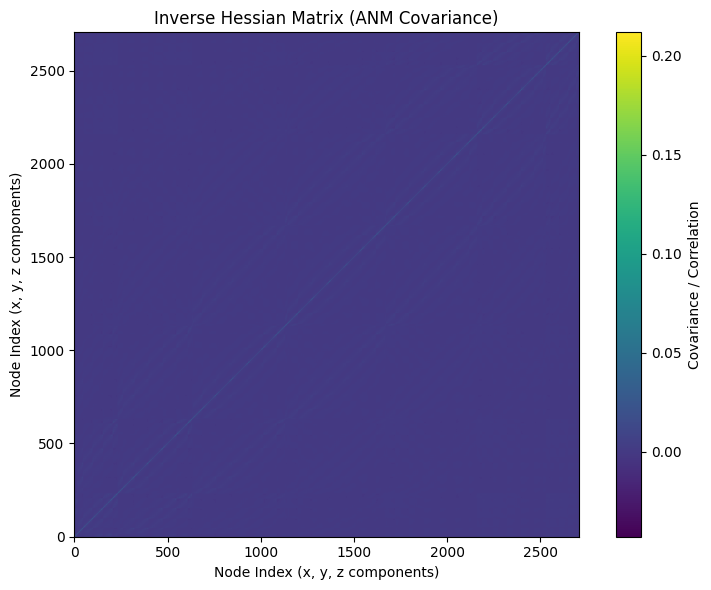
\includegraphics[width=0.8\textwidth]{Figure8-1.png}
  \caption{Inverse Hessian Matrix (ANM Covariance) with cutoff $R_c = 10.0$ \AA.}
  \label{fig:anm_hessian}
\end{figure}

\begin{figure}[htbp]
  \centering
  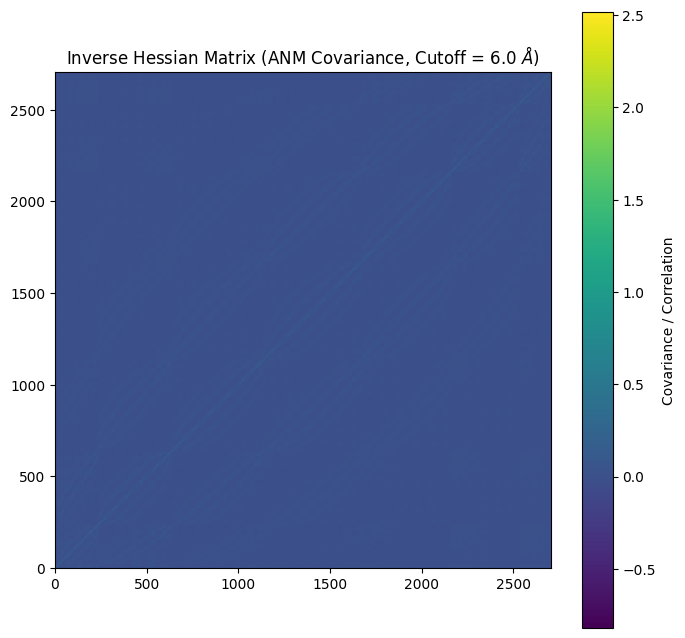
\includegraphics[width=0.8\textwidth]{Figure8-2.png}
  \caption{Inverse Hessian Matrix (ANM Covariance) with cutoff $R_c = 6.0$ \AA.}
  \label{fig:anm_hessian_6}
\end{figure}

\vspace{0.5cm}
\textbf{Information Provided by the Inverse Hessian Matrix:}\\
The inverse Hessian matrix functions as the 3D covariance (cross-correlation) matrix of the entire nanoparticle. It is a massive $3N \times 3N$ matrix. The intensely bright diagonal represents the perfect auto-correlation and mean-square fluctuations of individual nodes in 3D space.

The off-diagonal regions indicate the dynamic correlations between pairs of nodes across the x, y, and z axes. Positive values show that nodes are moving cooperatively in the same direction, while negative values indicate opposing (anti-correlated) motions. The repeating ``echo'' patterns visible throughout the matrix illustrate how atoms that are mathematically far apart in the sequence strongly influence each other due to their physical proximity on the 3D surface of the spherical quantum dot.

Comparing the two cutoff distances, the overall correlation patterns remain qualitatively similar, which is consistent with our earlier observation that the nanoparticle's tightly packed crystal lattice is not affected by the cutoff distance in terms of the eigenvalue structure. The primary difference is one of scale: the covariance magnitudes are larger for the $R_c = 6.0$ \AA\ case because fewer virtual springs result in a softer overall system, allowing greater fluctuations. This further confirms that for this nanoparticle, unlike typical proteins, the cutoff distance primarily controls the stiffness of the model rather than its connectivity or the qualitative nature of the vibrational modes.

\newpage

% ==========================================
% QUESTION 9
% ==========================================
\section*{ANM Construction and Results (Continued)}
\addcontentsline{toc}{section}{ANM Construction and Results (Continued)}

\textbf{Visualize directions/magnitudes of the motions associated with the lowest two modes; you may do so by using VMD’s \texttt{Extensions -> Analysis -> Normal Mode Wizard} once you generate \texttt{.nmd} files from Prody.}
\vspace{0.5cm}

Using the `.nmd` file generated from the ProDy calculations, the physical directions and magnitudes of the lowest two vibrational modes were visualized in VMD's Normal Mode Wizard. The green arrows indicate the specific 3D vectors of atomic displacement. In addition to the slowest modes, one of the highest frequency modes was also analyzed (Figure \ref{fig:vmd_mode3}). As seen in the image, the motion of the nodes is predominantly localized in the center of the nanoparticle. This structural behavior highlights that while it is relatively easy to induce motion in the unconstrained surface atoms, the tightly packed central atoms are significantly harder to move and vibrate.

\begin{figure}[htbp]
  \centering
  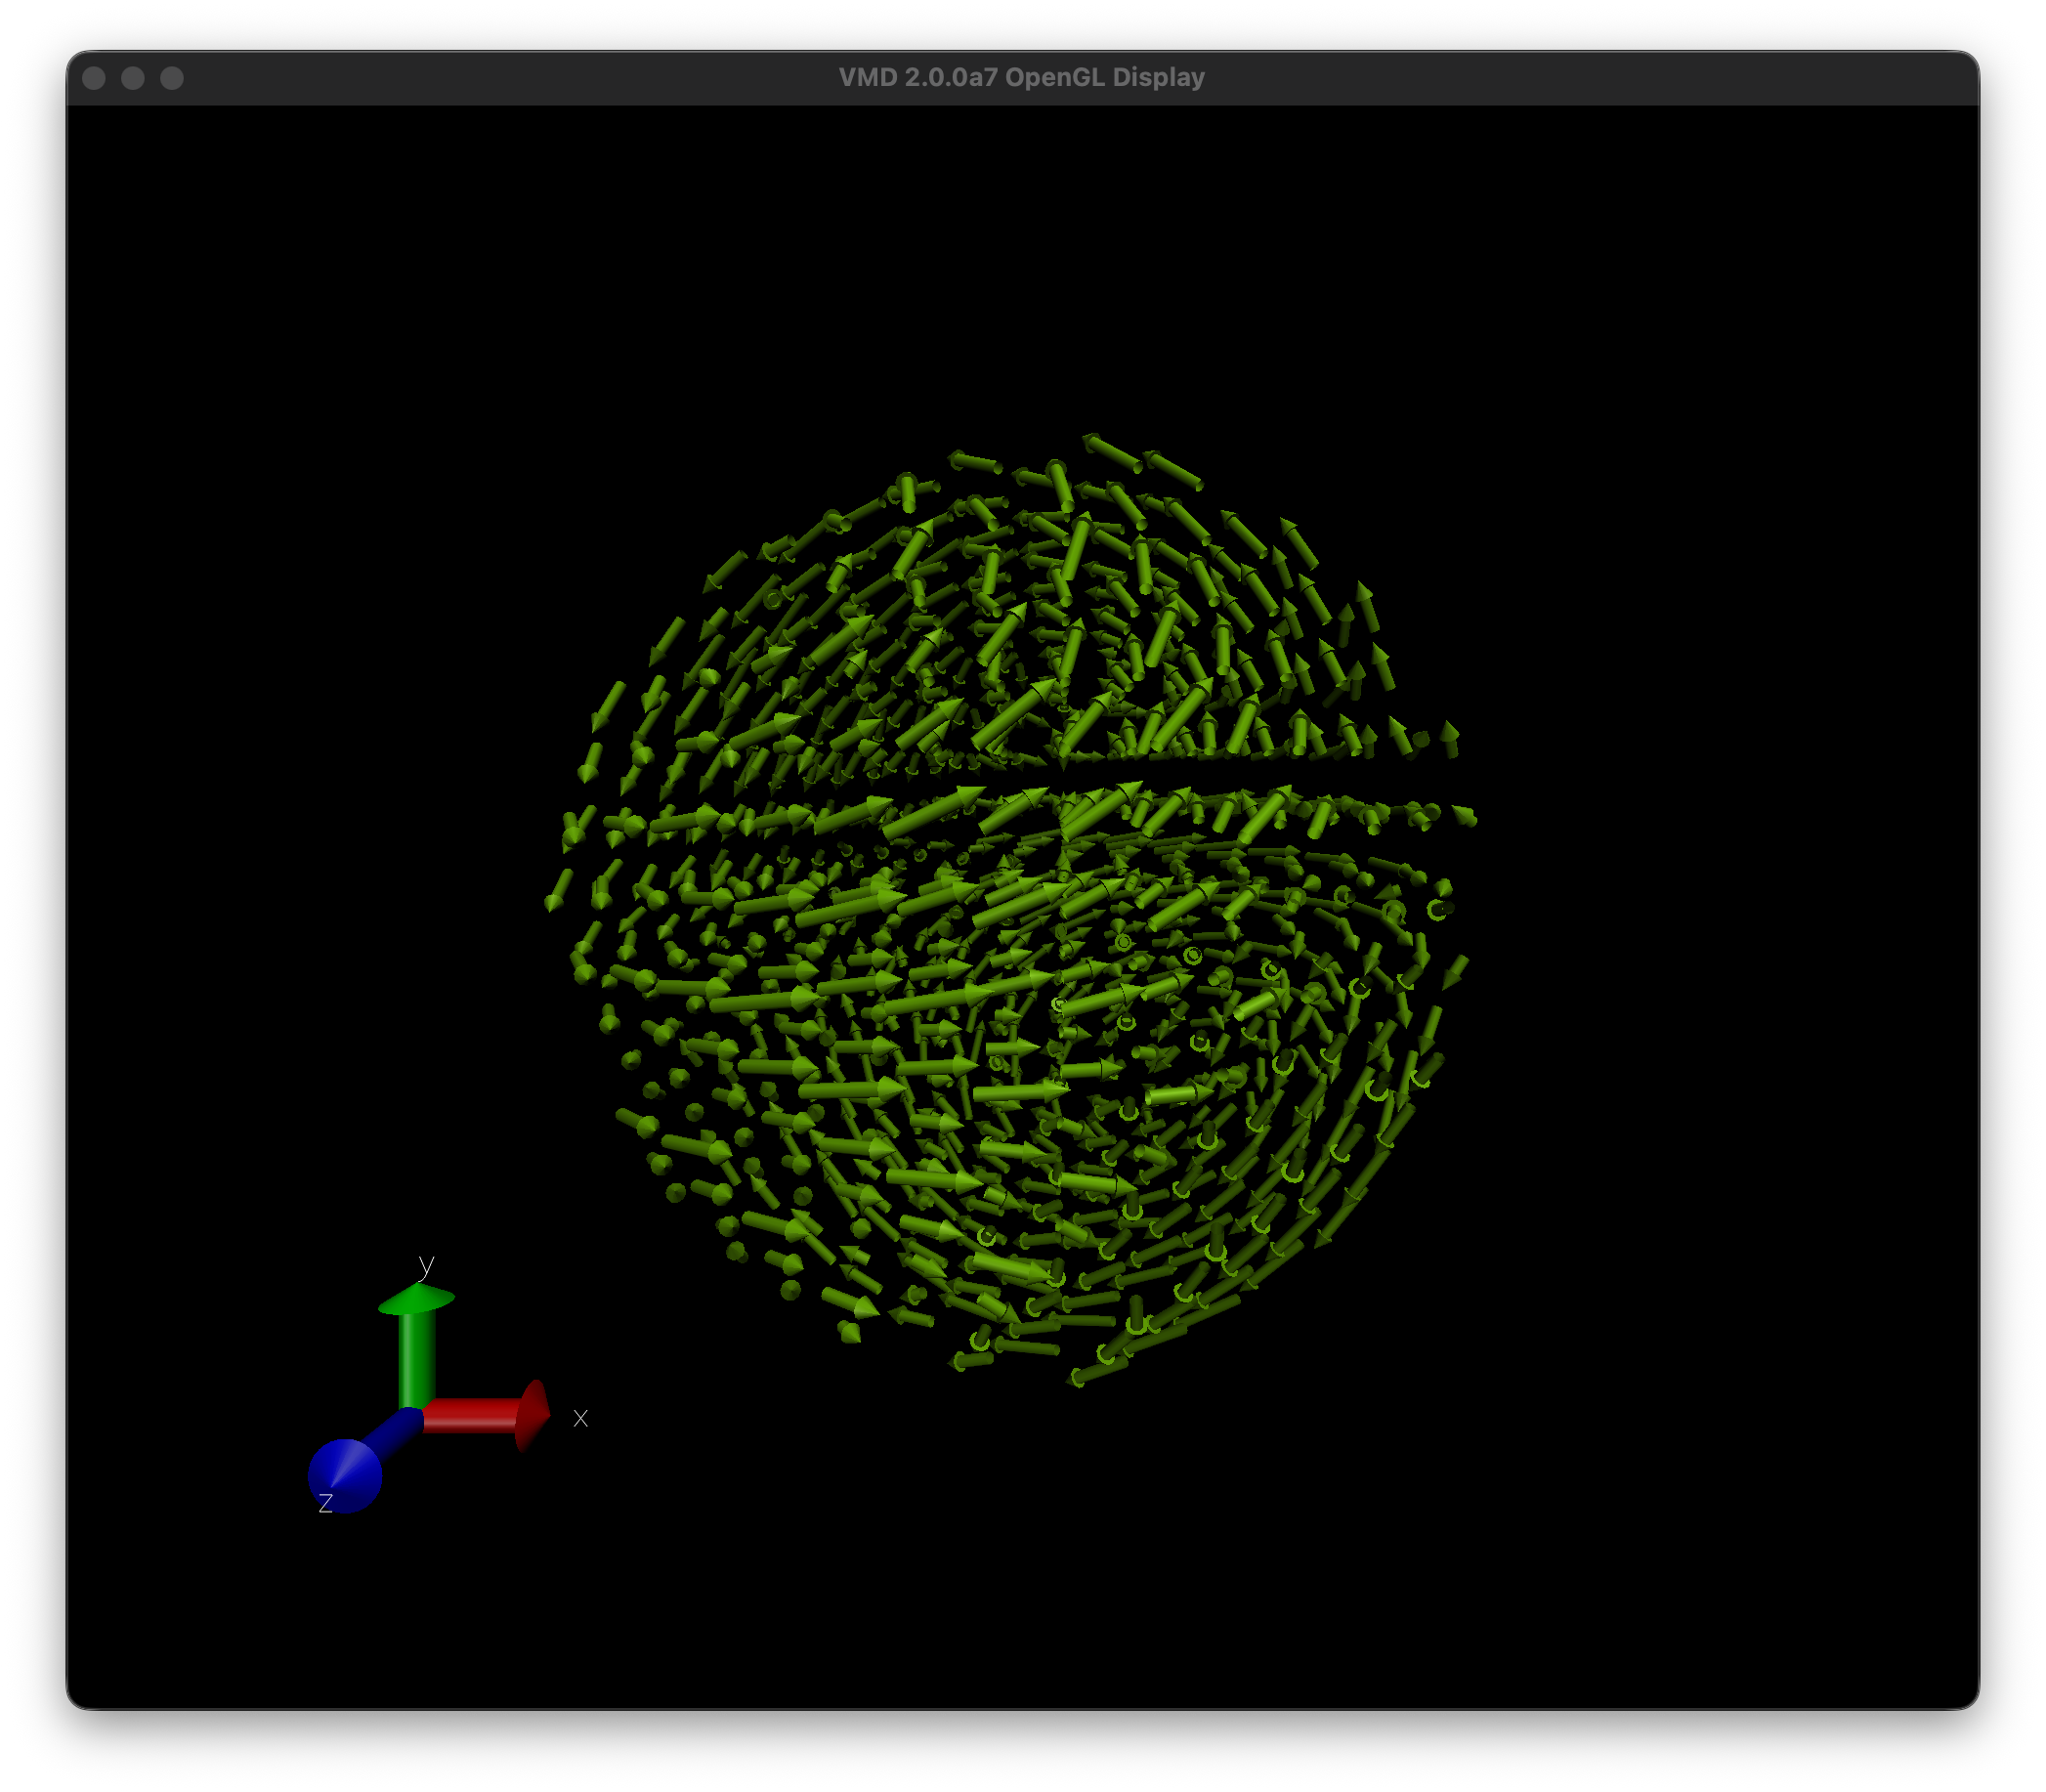
\includegraphics[width=0.8\textwidth]{Figure9-1.png}
  \caption{Visualization of Mode 1 (slowest mode) displaying global, cooperative surface motion.}
  \label{fig:vmd_mode1}
\end{figure}

\begin{figure}[htbp]
  \centering
  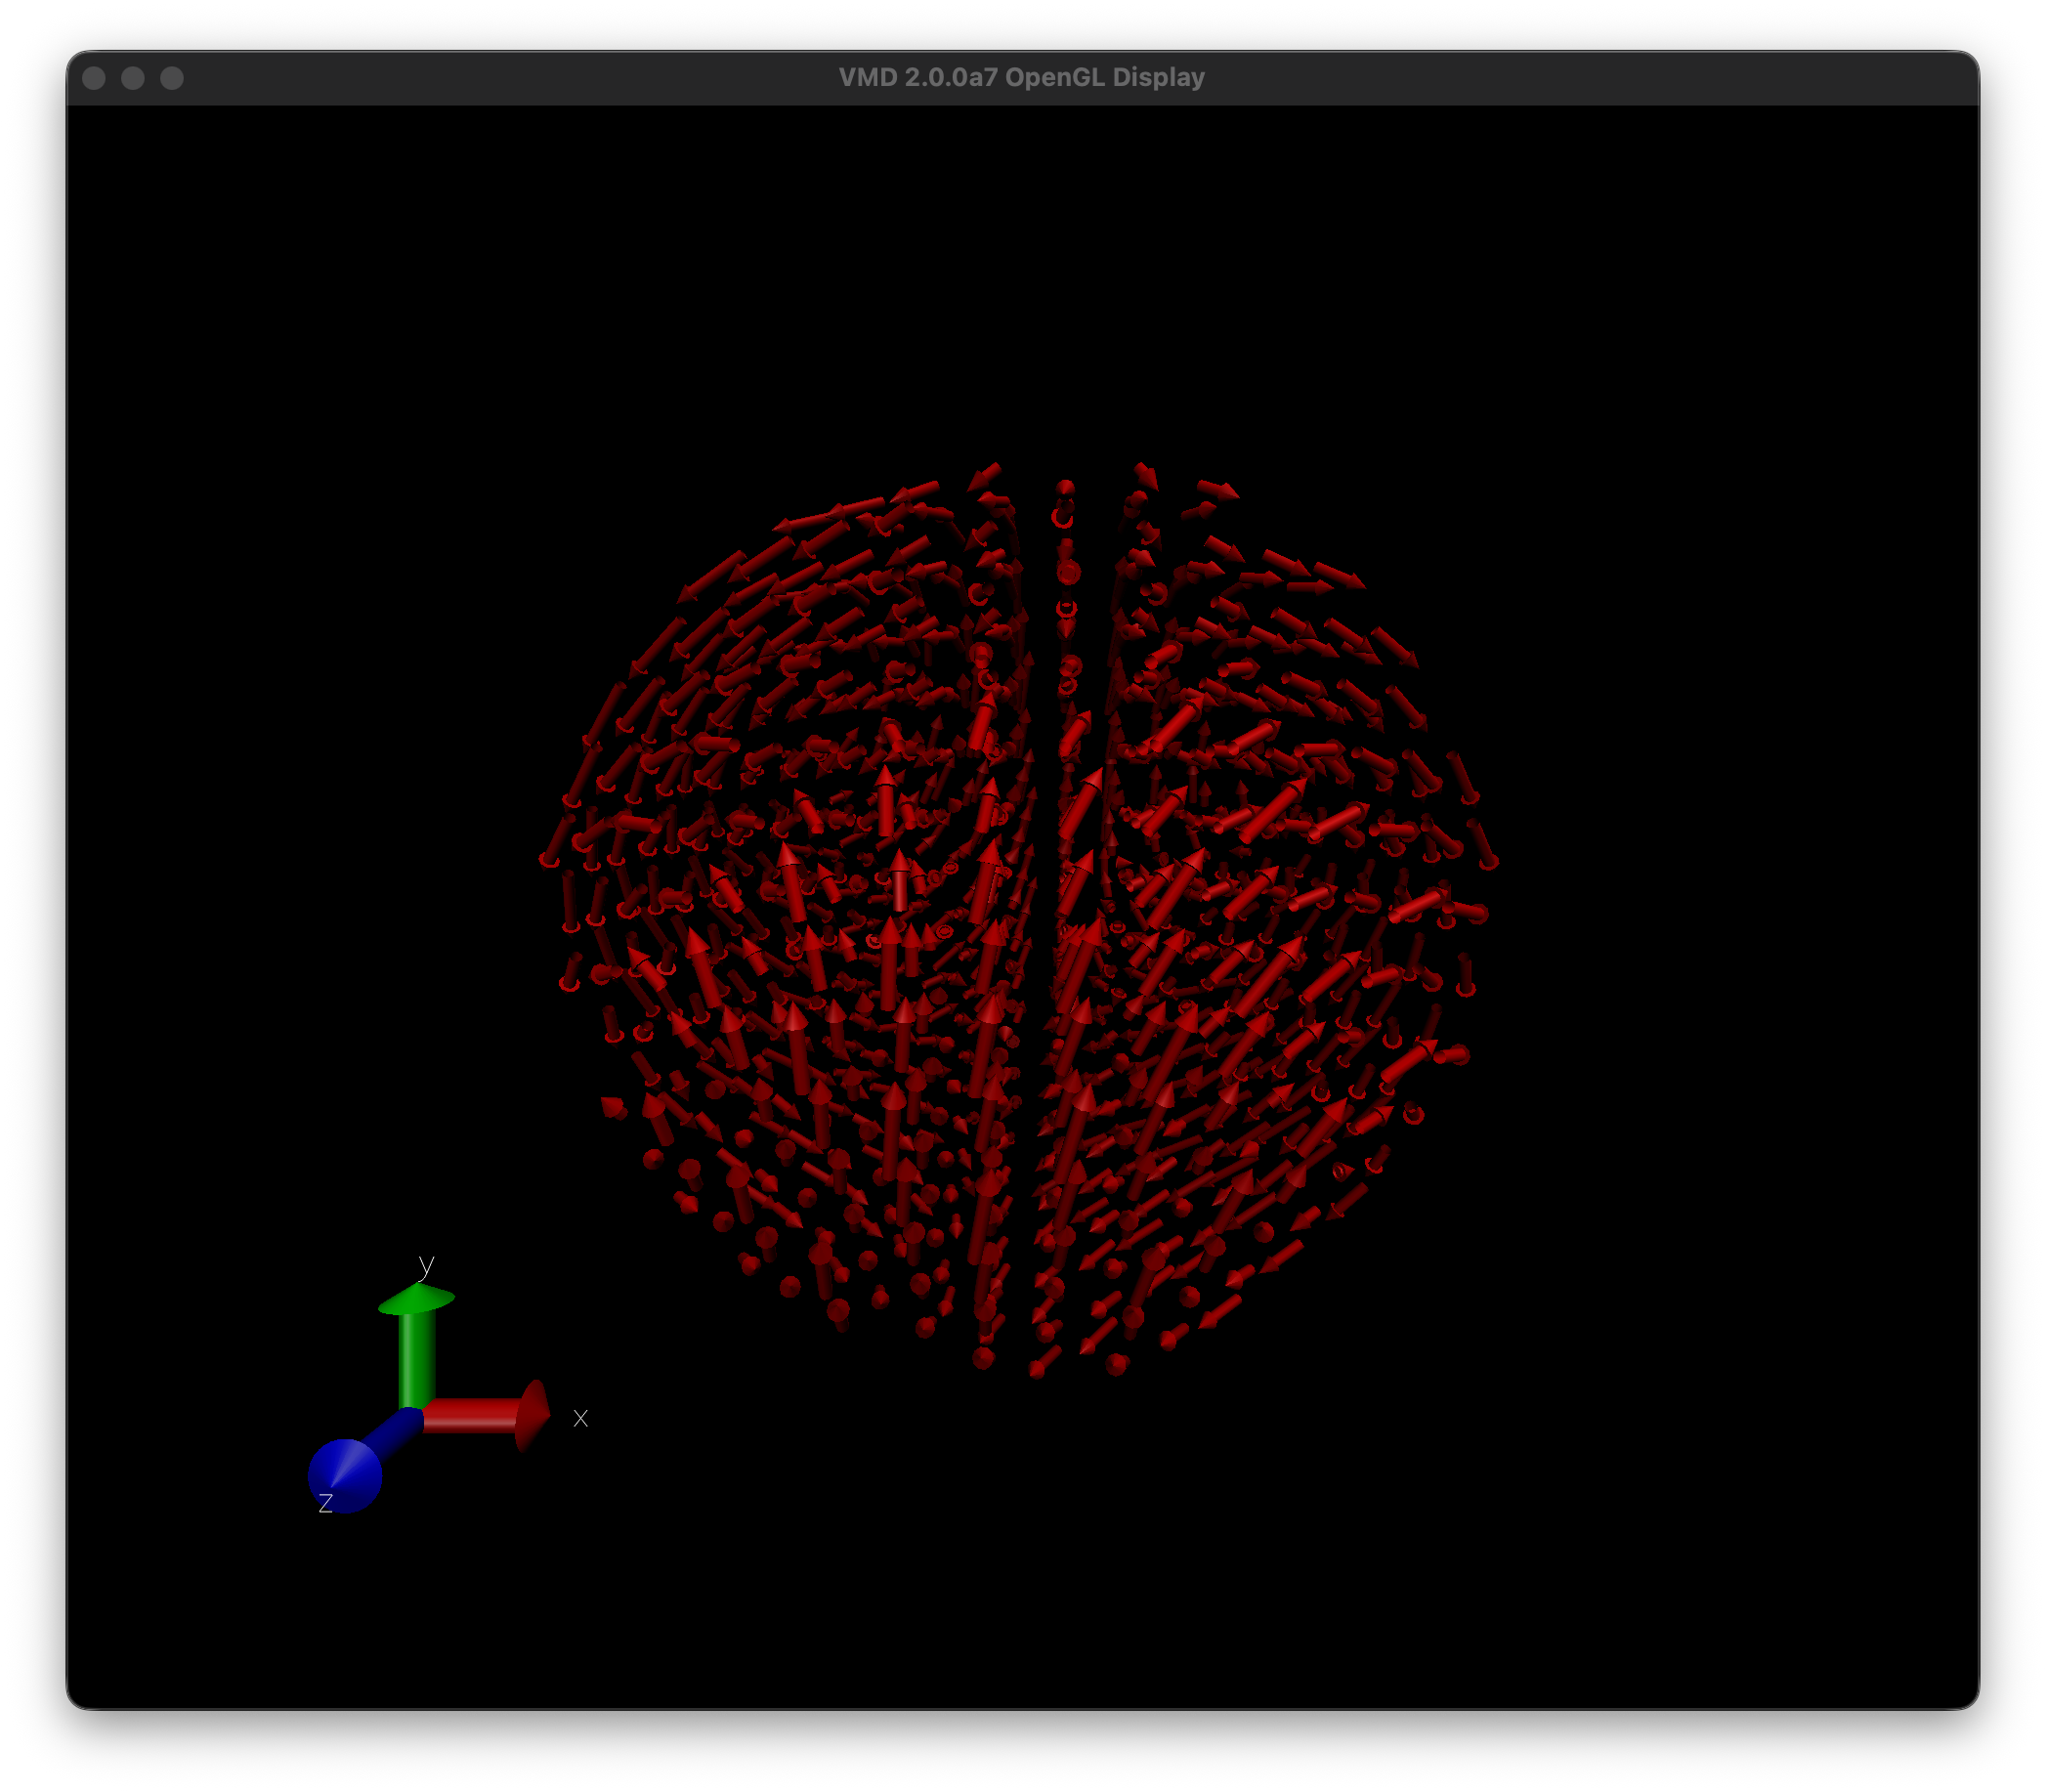
\includegraphics[width=0.8\textwidth]{Figure9-2.png}
  \caption{Visualization of Mode 2 displaying the second lowest-energy global deformation pattern.}
  \label{fig:vmd_mode2}
\end{figure}

\begin{figure}[htbp]
  \centering
  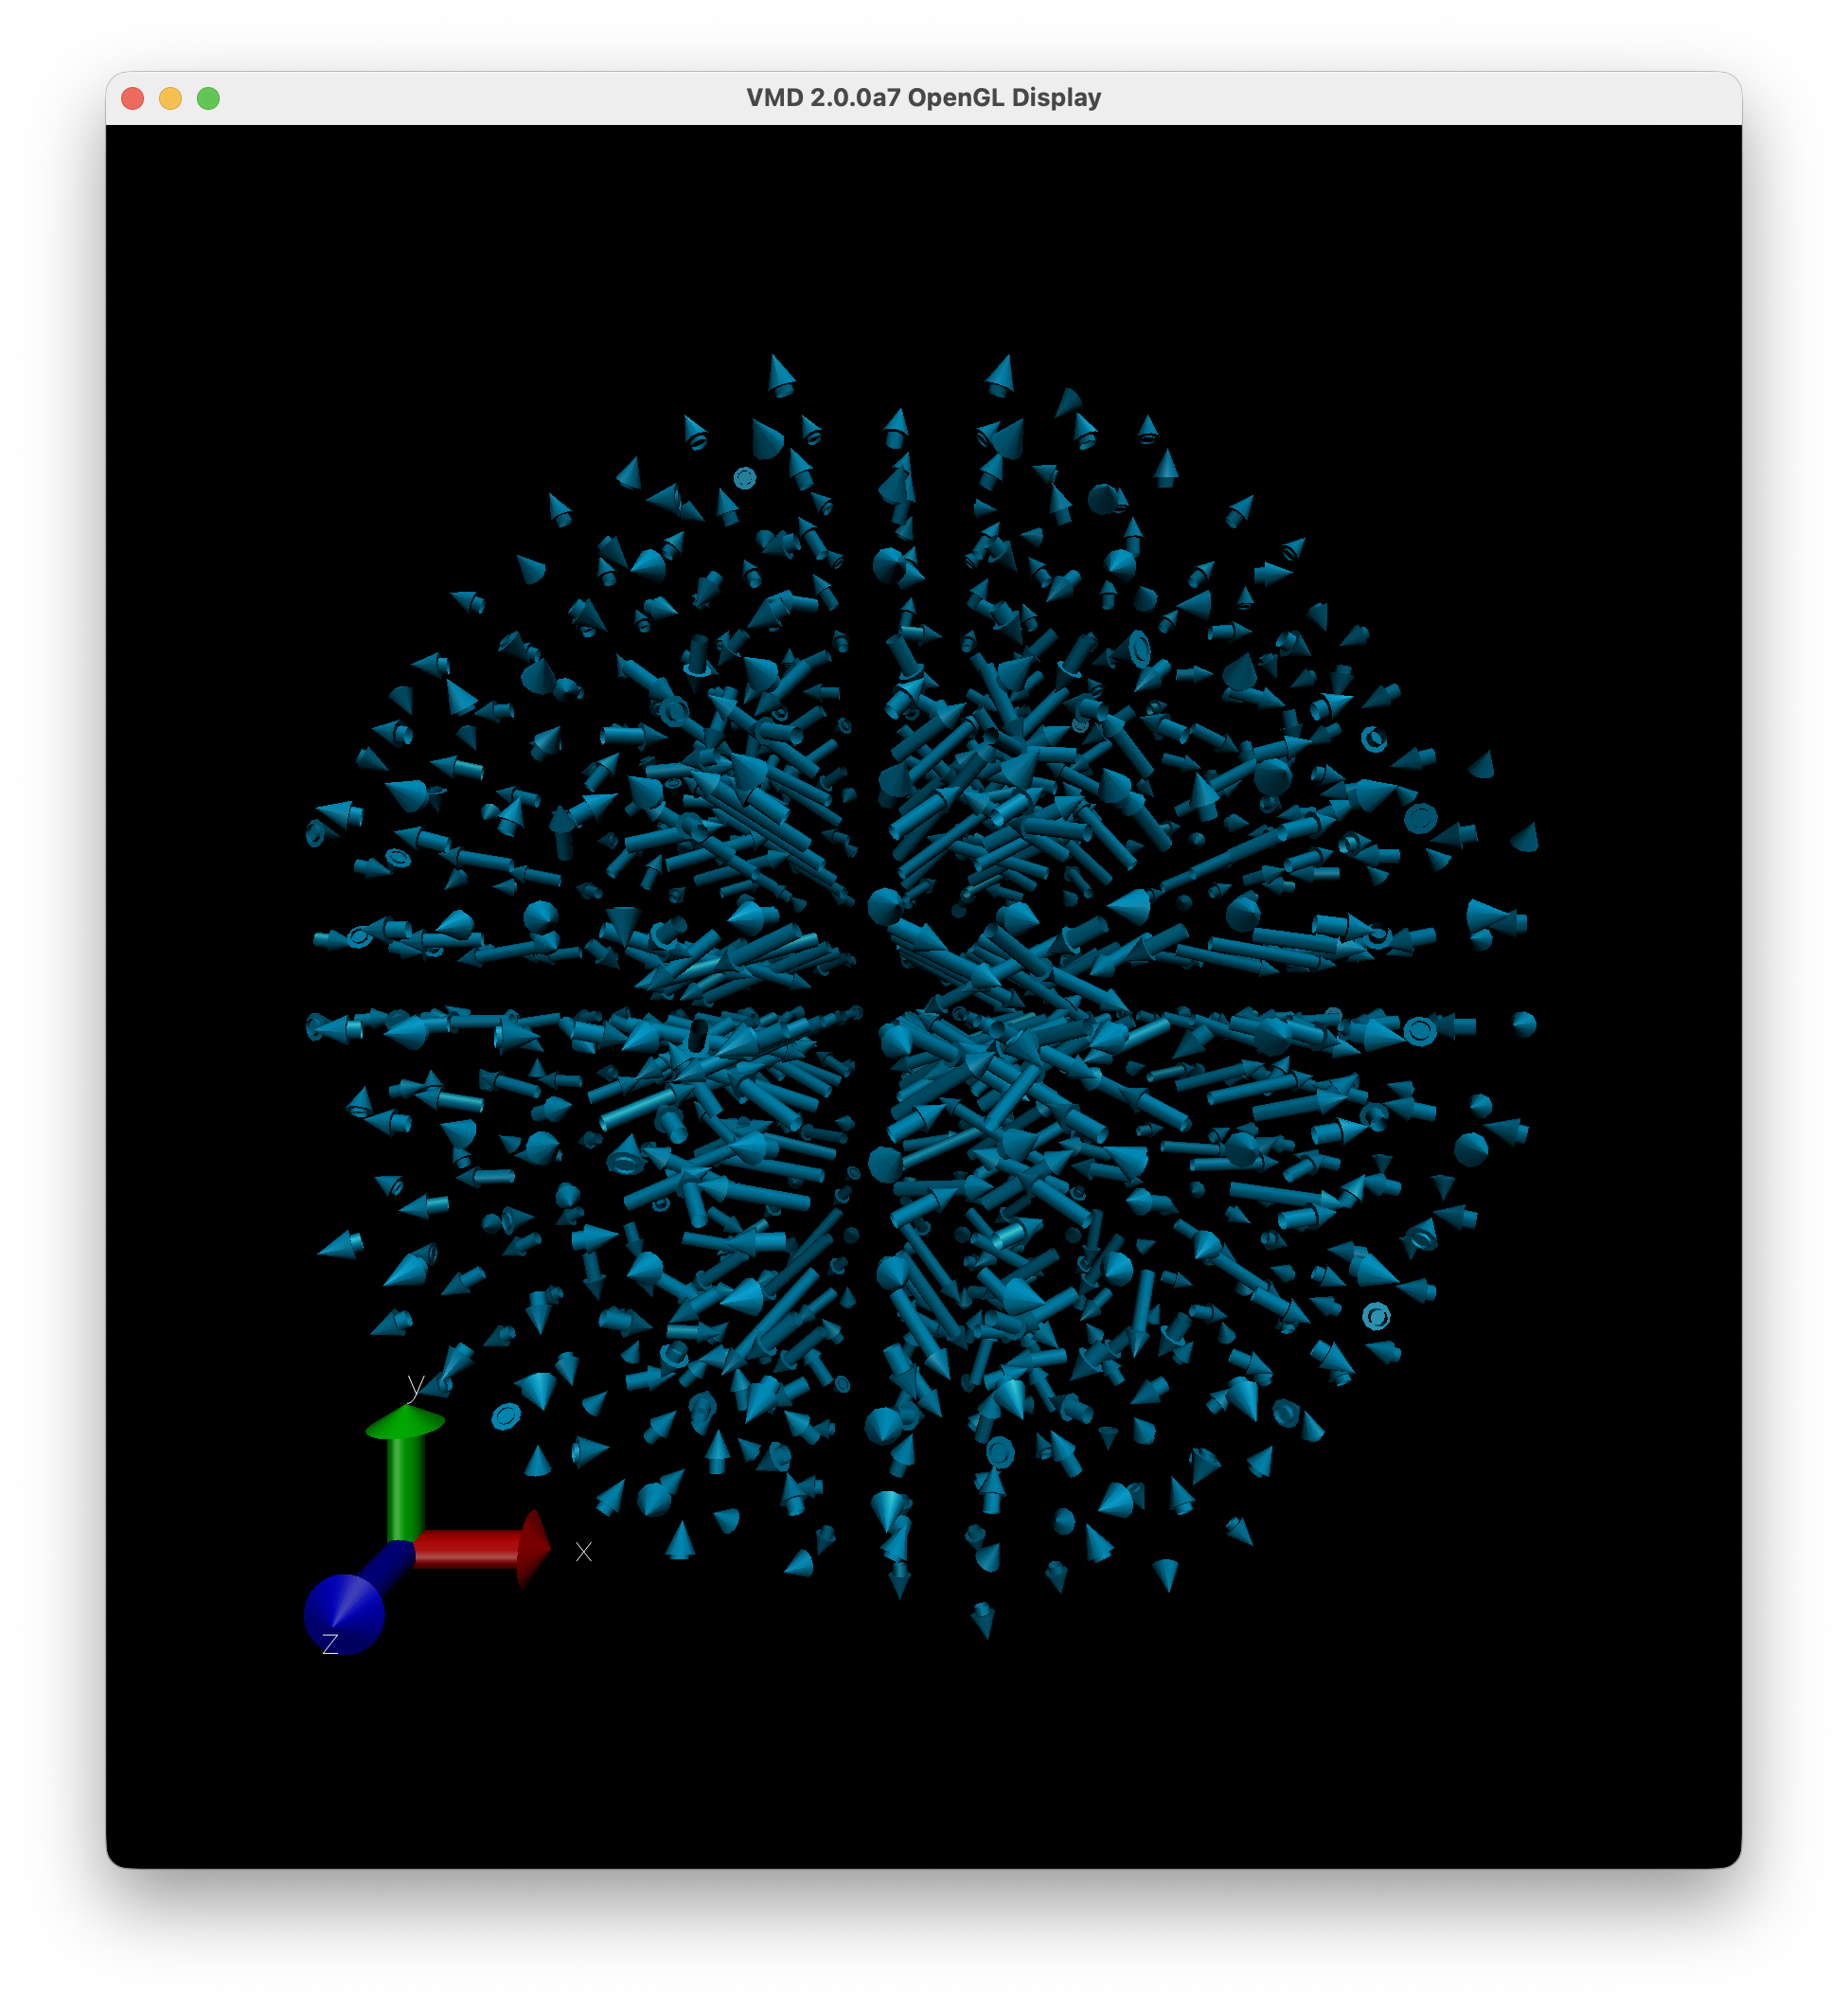
\includegraphics[width=0.8\textwidth]{Figure9-3.png}
  \caption{Visualization of one of the highest frequency modes, displaying highly localized vibrations predominantly in the rigid core of the nanoparticle.}
  \label{fig:vmd_mode3}
\end{figure}

\newpage

% ==========================================
% QUESTION 10
% ==========================================
\section*{Final Remarks}
\addcontentsline{toc}{section}{Final Remarks}

\textbf{Looking at all your findings, in a maximum of 80 words comment on how this nanoparticle might function.}
\vspace{0.5cm}

The normal mode analysis reveals that the CdTe quantum dot possesses a highly stable, tightly-packed core (demonstrated by high-frequency, localized modes) and a highly flexible outer shell (demonstrated by low-frequency, global bending/breathing modes). Functionally, this structural dynamic is ideal for display technologies or biological imaging: the rigid core ensures consistent, degradation-resistant light emission, while the flexible, highly mobile surface domains allow the nanoparticle to safely adapt, bind, and interact with surrounding solvents or ligands without fracturing.

\end{document}